
\documentclass[aspectratio=169]{beamer}
\usetheme{metropolis}           % Use metropolis theme
\usepackage[utf8]{inputenc}
\usepackage{graphicx}
\usepackage{eso-pic}
\usepackage{graphics}
\usepackage{tikz}
\usepackage[export]{adjustbox}
\usepackage{multicol}
\usepackage{listings}
\usepackage{helvet}
\usepackage{booktabs}
\usepackage{threeparttable}
\usepackage{fontspec}
\usepackage{hyperref}
\hypersetup{urlcolor=DarkBlue}

\title{Topic 7 - Track 1 \newline Data Visualization}
\date{\today}
\author{Author of Session here!} % Name of author(s) of session here
\institute{Development Impact Evaluation (DIME) \newline The World Bank }
\setbeamercolor{background canvas}{bg=white}	% Sets background color

% The below command places the World Bank logo and DIME logo to the right corner
\titlegraphic{%
	\begin{picture}(0,0)
	\put(330,-180){\makebox(0,0)[rt]{
\includegraphics[width=3cm]{../../img/WB_logo}}}
	\end{picture}%
	\begin{picture}(0,0)
	\put(390,-180){\makebox(0,0)[rt]{
\includegraphics[width=1.5cm]{../../img/i2i}}}
	\end{picture}%
}

%%% Section page with picture of Light bulb
\makeatletter
\defbeamertemplate*{section page}{mytheme}[1][]{
	\centering
	\begin{minipage}{22em}
		\raggedright
		\usebeamercolor[fg]{section title}
		\usebeamerfont{section title}
		\par
		\ifx\insertsubsectionhead\@empty\else%
		\usebeamercolor[fg]{subsection title}%
		\usebeamerfont{subsection title}%
		\fi
		\ifstrempty{#1}{}{%
			\includegraphics[width=100mm, height=60mm]{#1}%
		}
		\insertsectionhead\\[-1ex]
		\insertsubsectionhead
		\usebeamertemplate*{progress bar in section page}

	\end{minipage}
	\par
	\vspace{\baselineskip}
}
\makeatother

%%% Define a command to include picture in section,
%%% make section, and revert to old template
\newcommand{\sectionpic}[2]{
	\setbeamertemplate{section page}[mytheme][#2]
	\section{#1}
	\setbeamertemplate{section page}[mytheme]
}

%%% The command below allows for the text that contains Stata code
\lstset{ %
	backgroundcolor=\color{white},
	basicstyle=\tiny,
	breakatwhitespace=false,
	breaklines=true,
	captionpos=b,
	commentstyle=\color{mygreen},
	escapeinside={\%*}{*)},
	extendedchars=true,
	frame=single,
	numbers=left,
	numbersep=5pt,
	numberstyle=\tiny\color{gray},
	rulecolor=\color{black},
	showspaces=false,
	showstringspaces=false,
	showtabs=false,
	stringstyle=\color{mymauve},
	tabsize=2,
	title=\lstname,
	morekeywords={not,\},\{,preconditions,effects },
	deletekeywords={time}
}

\usepackage{fancyvrb} % Allows customization of verbatim environments
%Fancyvrb docs: http://mirrors.ibiblio.org/CTAN/macros/latex/contrib/fancyvrb/doc/fancyvrb-doc.pdf
\fvset{fontsize=\scriptsize} % The font size of all verbatim text can be changed here

%So we can use option FloatBarrier, which is similar to [H] but is an
%alternative solition when the algorithm can't solce [H] as too many
%settings are going on. [H] seems to get stuck in infinite loop
%https://tex.stackexchange.com/questions/2275/keeping-tables-figures-close-to-where-they-are-mentioned
\usepackage{placeins}
\newcommand{\codeexample}[2]{
	\begin{figure}
		\VerbatimInput[
		framesep=3mm,
		frame=lines, % line above and below code section
		numbers=left, %Line number
		label= #1, %name of code section
		baselinestretch=0.90, %Use line space more similat to line space in code editors
		]{#2} %Write the relative file path and the name of the file to be included
	\end{figure}
	\FloatBarrier
}



%% The below command creates the ligh bulb logos in the top right corner of the
\begin{document}

	{
		\usebackgroundtemplate{
\includegraphics[height=55mm, right]{../../img/top_right_corner.pdf}}
		\maketitle
	}

%%%%%%%%%%%%%%%%%%%%%%%%%%%%%%%%%%%%%%%%%%% heading of section 1
\begin{frame}[fragile]{Tables give all the details}
	\begin{columns}[c]
		\column{.30\textwidth}
		\begin{itemize}
			\item What’s happening in this regression table?
			\item What’s important?
		\end{itemize}
		\column{.70\textwidth}
		\begin{figure}
			\centering
			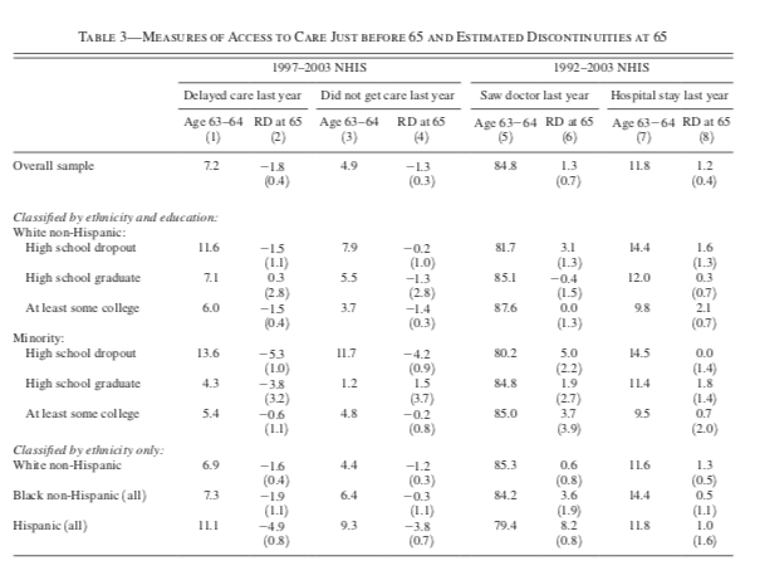
\includegraphics[width=\linewidth]{img/regtable}
		\end{figure}
	\end{columns}
\end{frame}

\begin{frame}[fragile]{But figures tell the story}
	\begin{columns}[c]
		\column{.35\textwidth}
		\begin{itemize}
			\item This is the data that generates those estimates.
			\item You can see exactly what is happening very quickly!
		\end{itemize}
		\column{.65\textwidth}
		\begin{figure}
			\centering
			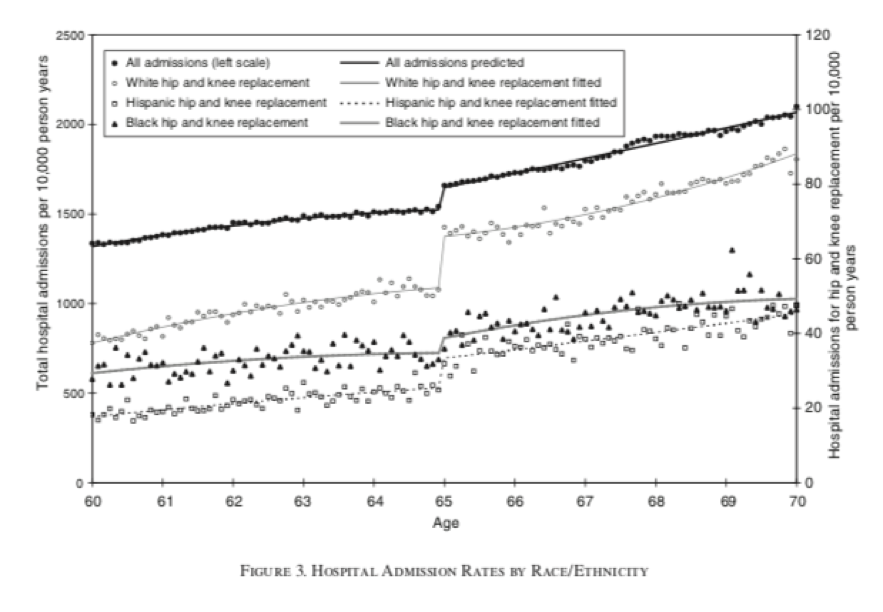
\includegraphics[width=\linewidth]{img/line}
		\end{figure}
	\end{columns}
\end{frame}

\begin{frame}[fragile]{Examples: comparing means}
	\begin{columns}[c]
		\column{.40\textwidth}
		\begin{itemize}
			\item What is the main story in this graph?
			\item We need more context to say something detailed about this, but what has the person creating the graph highlighted for us?
		\end{itemize}
		\column{.60\textwidth}
		\begin{figure}
			\centering
			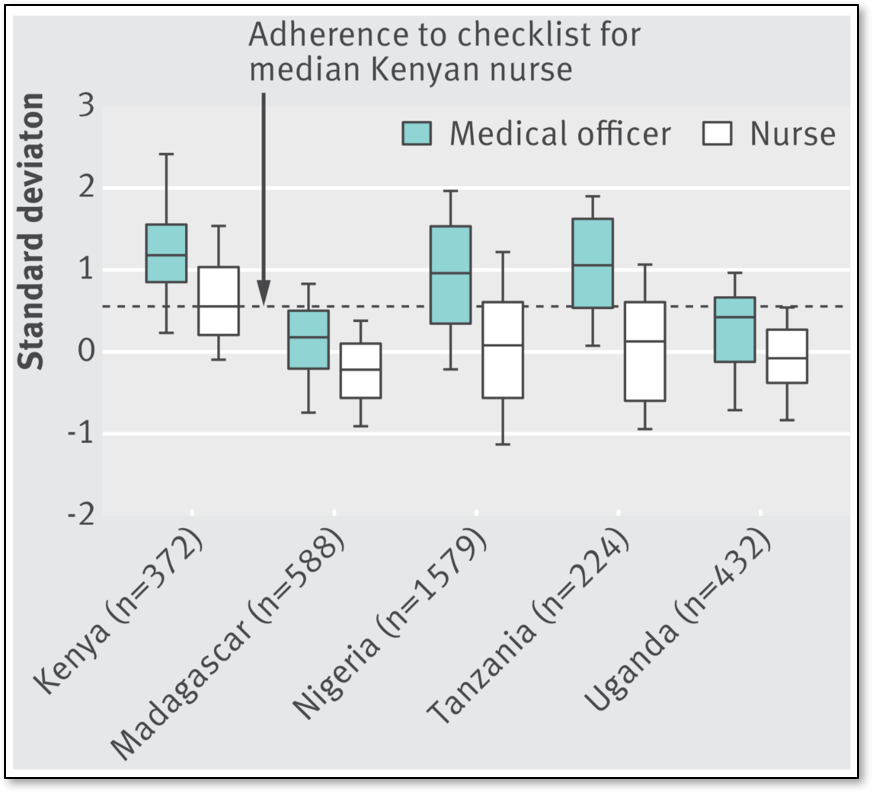
\includegraphics[width=\linewidth]{img/boxplot1}
		\end{figure}
	\end{columns}
\end{frame}

\begin{frame}{Stata Default Graphs}
	\begin{figure}
		\centering
		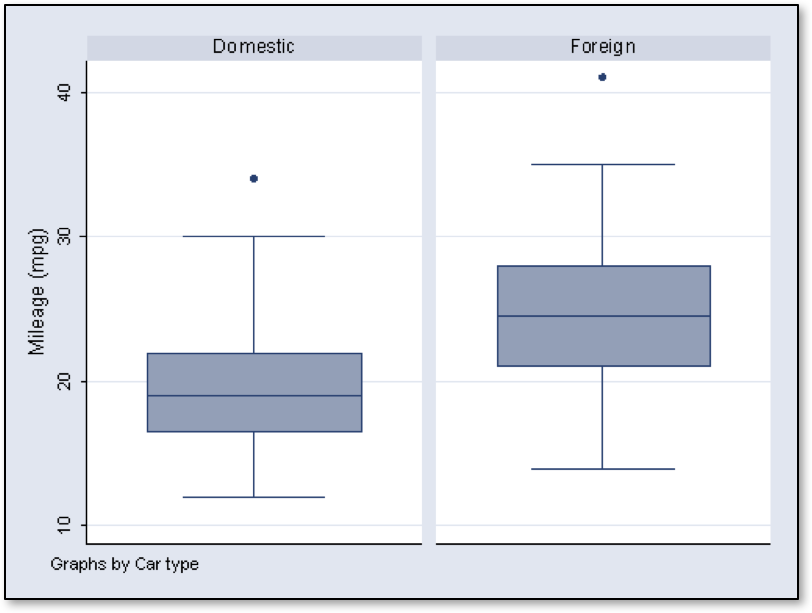
\includegraphics[width= 2 in]{img/boxplot2}
		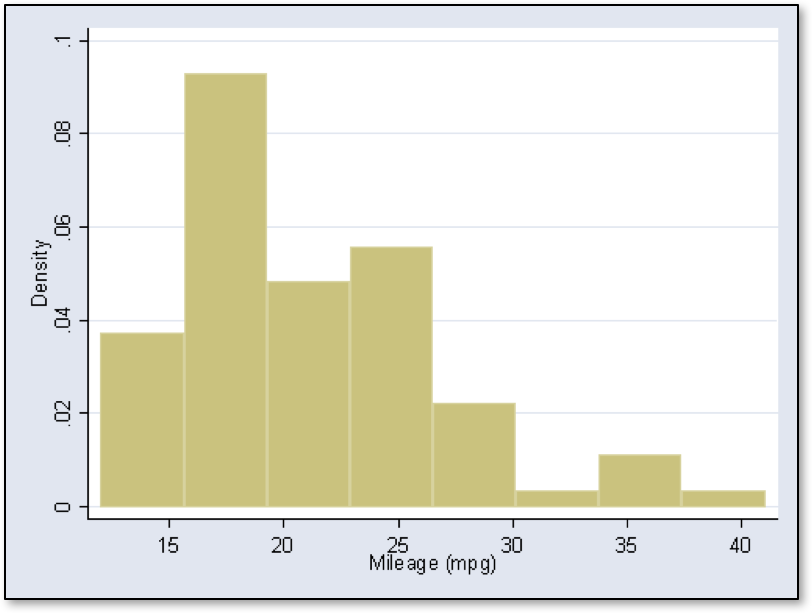
\includegraphics[width= 2 in]{img/histogram1}
		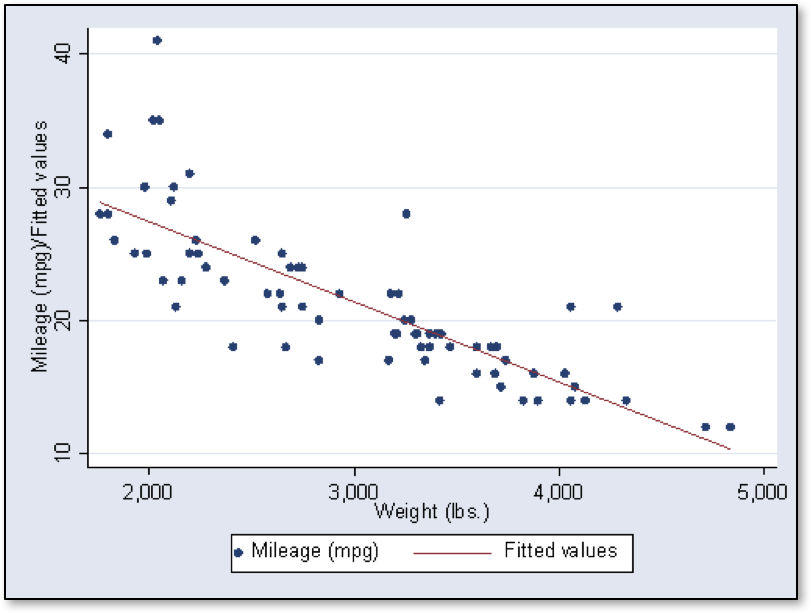
\includegraphics[width= 2 in]{img/scatter1}
	\end{figure}
\end{frame}

\begin{frame}[fragile]{Stata has three core built-in graph functions}
	\begin{columns}[c]
		\column{.40\textwidth}
		\begin{itemize}
			\item \texttt{graph graphtype} - graphs which plot one or more variables on one axis
			\item \texttt{twoway graphtype} - graphs which plot two variables together on an x,y axis
			\item \texttt{histogram}, \texttt{kdensity}, \texttt{lowess} - essential distributional commands
		\end{itemize}
		\column{.60\textwidth}
		\begin{figure}
			\centering
			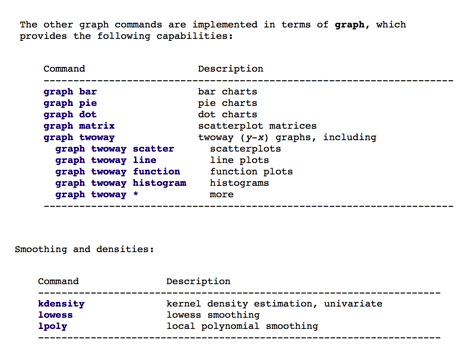
\includegraphics[width=\linewidth]{img/graphcommand}
		\end{figure}
	\end{columns}
\end{frame}

\begin{frame}[fragile]{[Oneway] graph plots can be very informative}
	\begin{columns}[c]
		\column{.50\textwidth}
		\begin{figure}
			\centering
			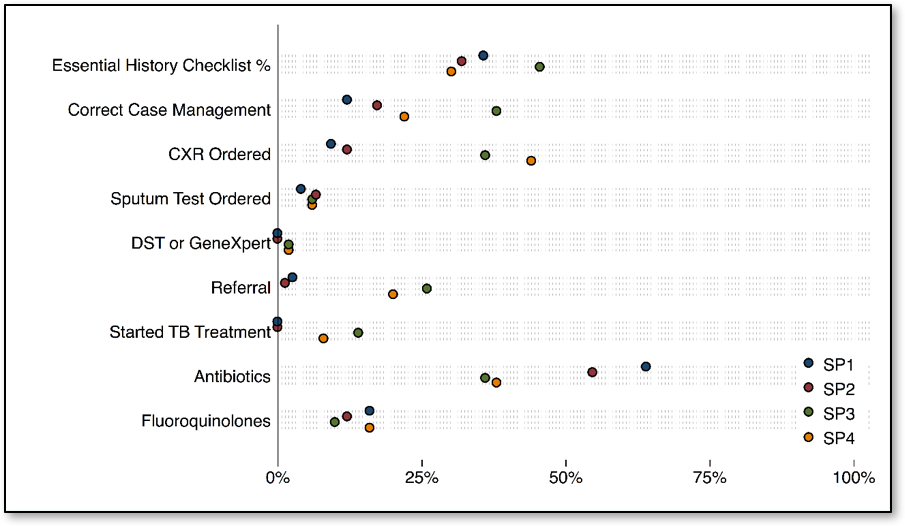
\includegraphics[width=\linewidth]{img/oneway1}
		\end{figure}
		Figure 1. \url{https://github.com/qutubproject/lancetid2015/blob/master/tables_figures.do}
		\column{.50\textwidth}
		\begin{figure}
			\centering
			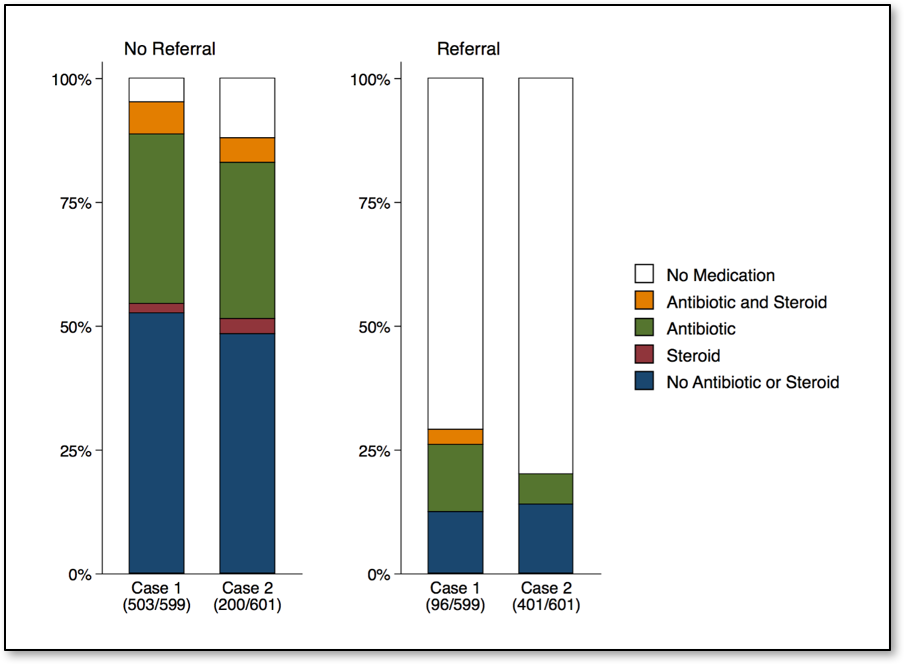
\includegraphics[width=\linewidth]{img/oneway2}
		\end{figure}
		Figure 2. \url{https://github.com/qutubproject/lancetid2016/blob/master/tables_figures.do}
	\end{columns}
\end{frame}

\begin{frame}[fragile]{[Twoway] graphs}
	\begin{columns}[c]
		\column{.50\textwidth}
		\begin{itemize}
			\item Each point in the graph represents a combination of the y-axis and the x-axis
			\item Can be many types of graphs. This is a scatter plot, but it can be areas, lines, bars, etc.
		\end{itemize}
		\column{.50\textwidth}
		\begin{figure}
			\centering
			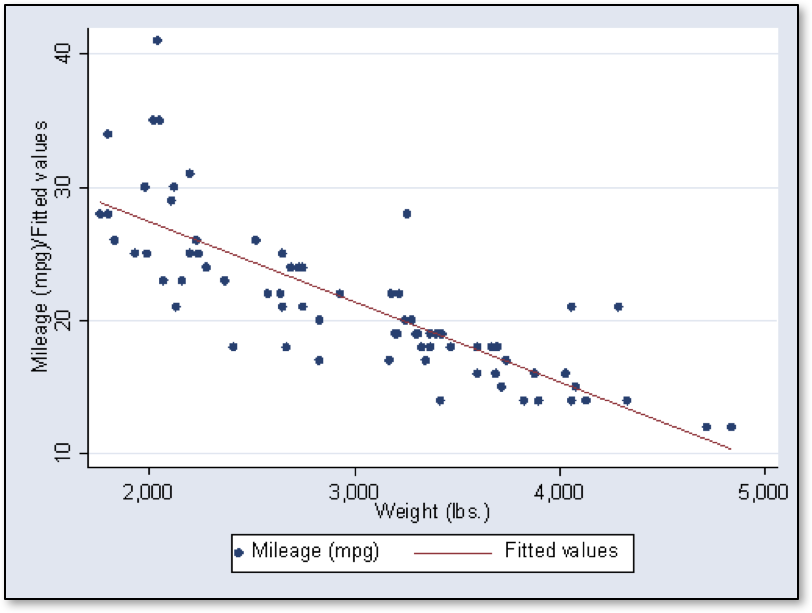
\includegraphics[width=\linewidth]{img/twoway1}
		\end{figure}
	\end{columns}
\end{frame}


\begin{frame}[fragile]{ Multiple [twoway] graphs in one graph}
	\begin{columns}[c]
		\column{.50\textwidth}
		\begin{itemize}
			\item You can add multiple graphs in the same graph and format the data points slightly differently
			\item \texttt{tw (type var1 var2 , opts) (type var3 var4 , opts), opts}
			\item More on this in Track 2
		\end{itemize}
		\column{.50\textwidth}
		\begin{figure}
			\centering
			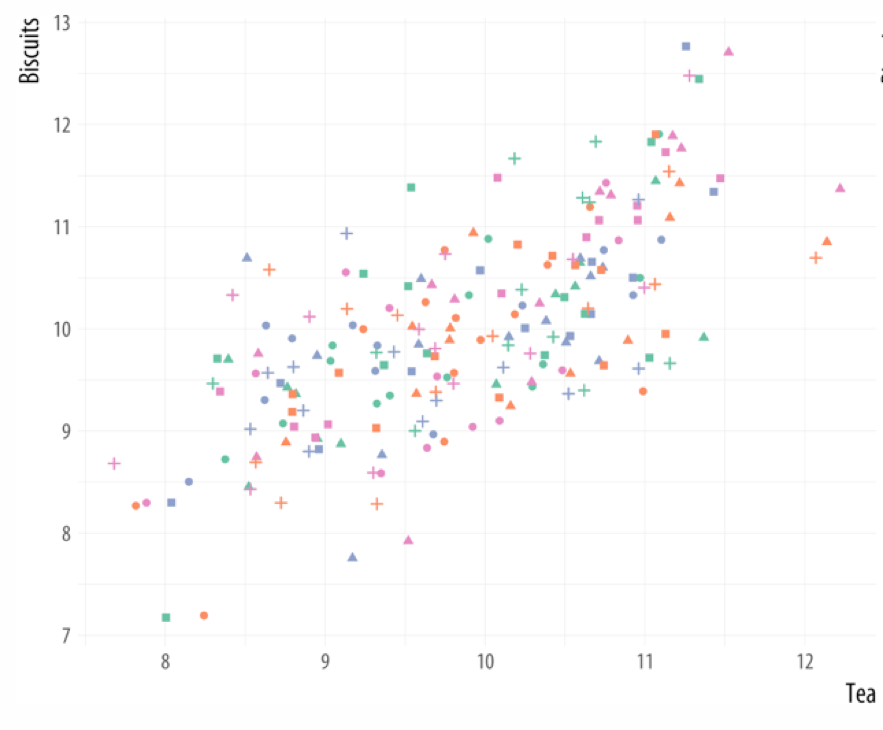
\includegraphics[width=\linewidth,frame]{img/twoway2}
		\end{figure}
	\end{columns}
\end{frame}

\begin{frame}[fragile]{Task 1 - Histogram}
	1. Create a histogram for the variable \texttt{ag\_16\_x\_16\_1}
	\codeexample{hist1.do}{code/hist1.do}
	
	2. Histograms are great to spot outliers. But we also want to use histograms to explore the distribution of the non-outlier observations. Find a reasonable range for values to do that.
	\codeexample{hist2.do}{code/hist2.do}
\end{frame}
  

 
\begin{frame}[fragile]{Task 1 - Histogram}
 
 	Make changes to the histogram to make it look presentable. Make the y-axis depict frequencies \& change the width of the bins
	\codeexample{hist3.do}{code/hist3.do}
 
 	Make more formatting edits and save the file. This code is in the example do-file so no need to re-type.
	\codeexample{hist4.do}{code/hist4.do}
 
\end{frame}


\begin{frame}[fragile]{Task 2 - Bar graph}
	1. Create a bar graph for the variable \texttt{ag\_17\_x\_16\_1}
	\codeexample{bar1.do}{code/bar1.do}
		
	2. Make changes to the bar graph to make it look presentable. Graph it over the various categories of \texttt{gr\_16}
	\codeexample{bar2.do}{code/bar2.do}

\end{frame}

\begin{frame}[fragile]{Task 2}
	\begin{itemize}
		\item Make changes to the bar graph to make it look nicer.
		\begin{itemize}
			\item Change the options for the titles and labels
			\item Change it to a horizontal bar graph
		\end{itemize}
		\item Save the final graph created
	\end{itemize}
	\codeexample{bar3.do}{code/bar3.do}
\end{frame}


\begin{frame}[fragile]{Task 3 - Scatter plots}
	Let's make a scatter plot for the variables \texttt{ag\_18\_x\_16\_1} and \texttt{ag\_16\_x\_16\_1} only for the control group
	\codeexample{scatter1.do}{code/scatter1.do}
\end{frame}

\begin{frame}[fragile]{Task 3 - Scatter plots}

	Add a fitted line to the last graph. Still only control.
	\codeexample{scatter2.do}{code/scatter2.do}
\end{frame}

\begin{frame}[fragile]{Task 3 - Scatter plots}		
	
	Include both treatment and control, but generate different scatter plot and lowess graphs in the same grpah so we can tell them apart. Then also save the final graph.
	\codeexample{scatter3.do}{code/scatter3.do}
\end{frame}


\begin{frame}[fragile]{Graphs can be combined and exported}
	\begin{columns}[c]
		\column{.50\textwidth}
		\begin{figure}
			\centering
			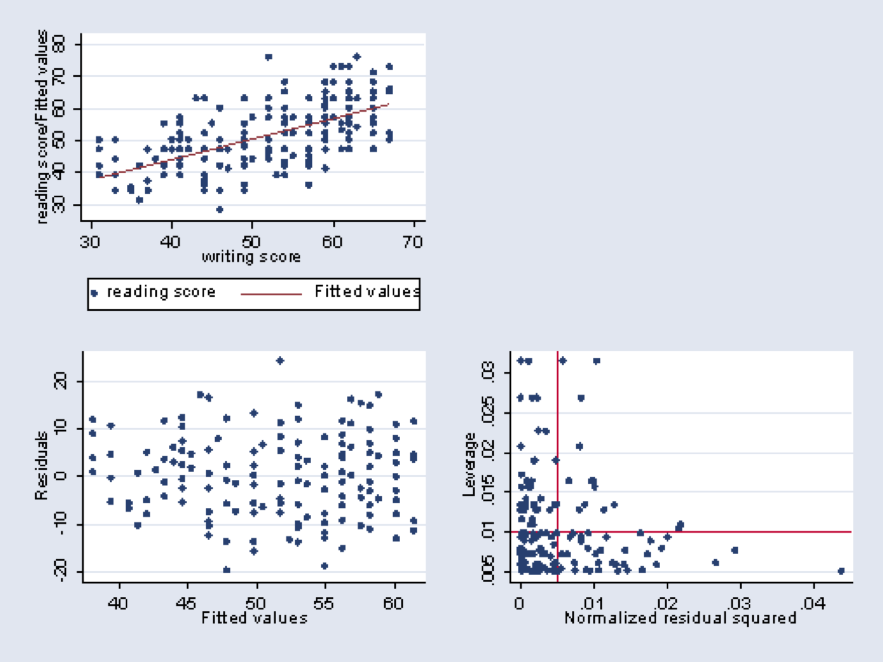
\includegraphics[width=\linewidth]{img/grcombine}
		\end{figure}

		\column{.50\textwidth}
		\begin{enumerate}
			\item \texttt{graph combine graph-1 graph-2 graph-3}
			\item \texttt{graph export “filename.png", replace}
		\end{enumerate}
		\begin{itemize}
			\item use .png or .eps
			\begin{itemize}
				\item With .png, specify \texttt{width(1000)} for higher resolution
				\item .eps files can scale to any size on most modern software (but hard to preview in older systems)
			\end{itemize}
		\end{itemize}
	\end{columns}
\end{frame}

\begin{frame}[fragile]{Task 4 - Combining graphs}
	\begin{itemize}
		\item Combine the histogram, bar graph, and scatter plot created earlier in this exercise
		\item Save the combined graph as a png file
	\end{itemize}
	\codeexample{combine-graphs.do}{code/combine-graphs.do}
\end{frame}

\begin{frame}[fragile]{DIME Resources (please contribute!)}
	\begin{columns}[c]
		\column{.35\textwidth}
		\begin{figure}
			\centering
			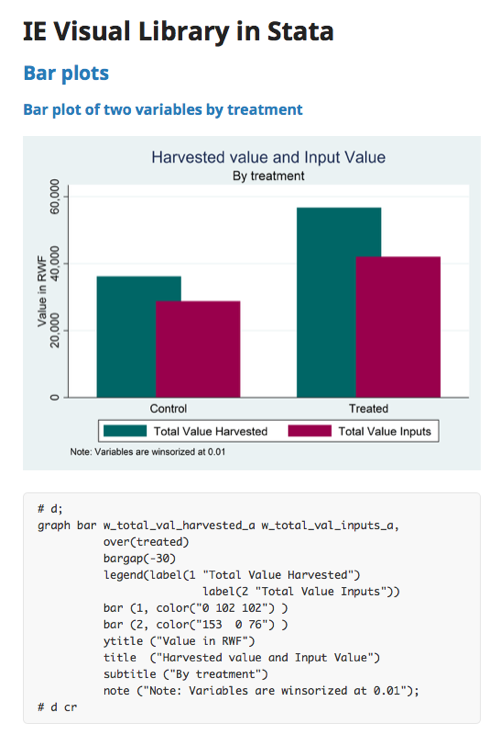
\includegraphics[width=\linewidth]{img/visualie}
		\end{figure}

		\column{.30\textwidth}

		\small <- \newline \url{https://worldbank.github.io/Stata-IE-Visual-Library/}

		\vspace{.8cm}

		\small -> \newline \url{https://worldbank.github.io/stata/}

		\column{.35\textwidth}
		\begin{figure}
			\centering
			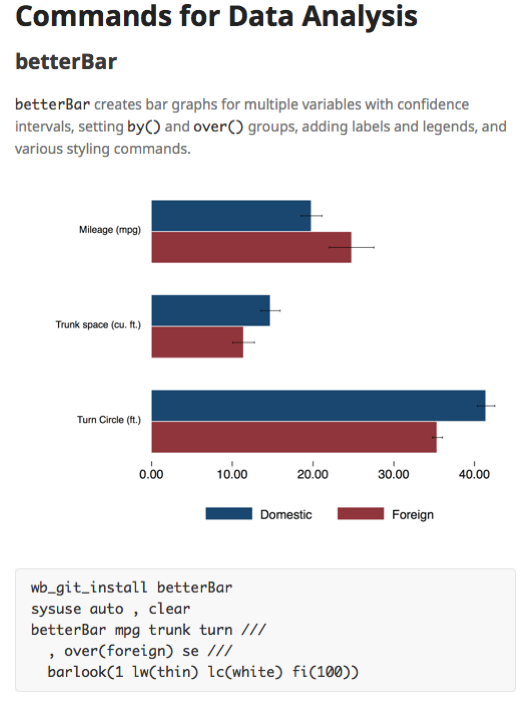
\includegraphics[width=\linewidth]{img/visualie2}
		\end{figure}
	\end{columns}
\end{frame}


%%%%%%%%%%%%%%%%%%%%%%%%%%%%%%%%%%%%%%%%%%% Final thougts section
\begin{frame}{Conclusion}


\vspace{20mm}
For more information or further questions please contact:
\newline John Doe (\url{johndoe@worldbank.org}) \newline Mary Doe (\url{marydoe@worldbank.org})

\end{frame}

%%%%%%%%%%%%%%%%%%%%%%%%%%%%%%%%%%%%%%%%%%% The End
\sectionpic{Thank You!}{../../img/section_slide}






\end{document}
